\thispagestyle{empty}
\begin{center}
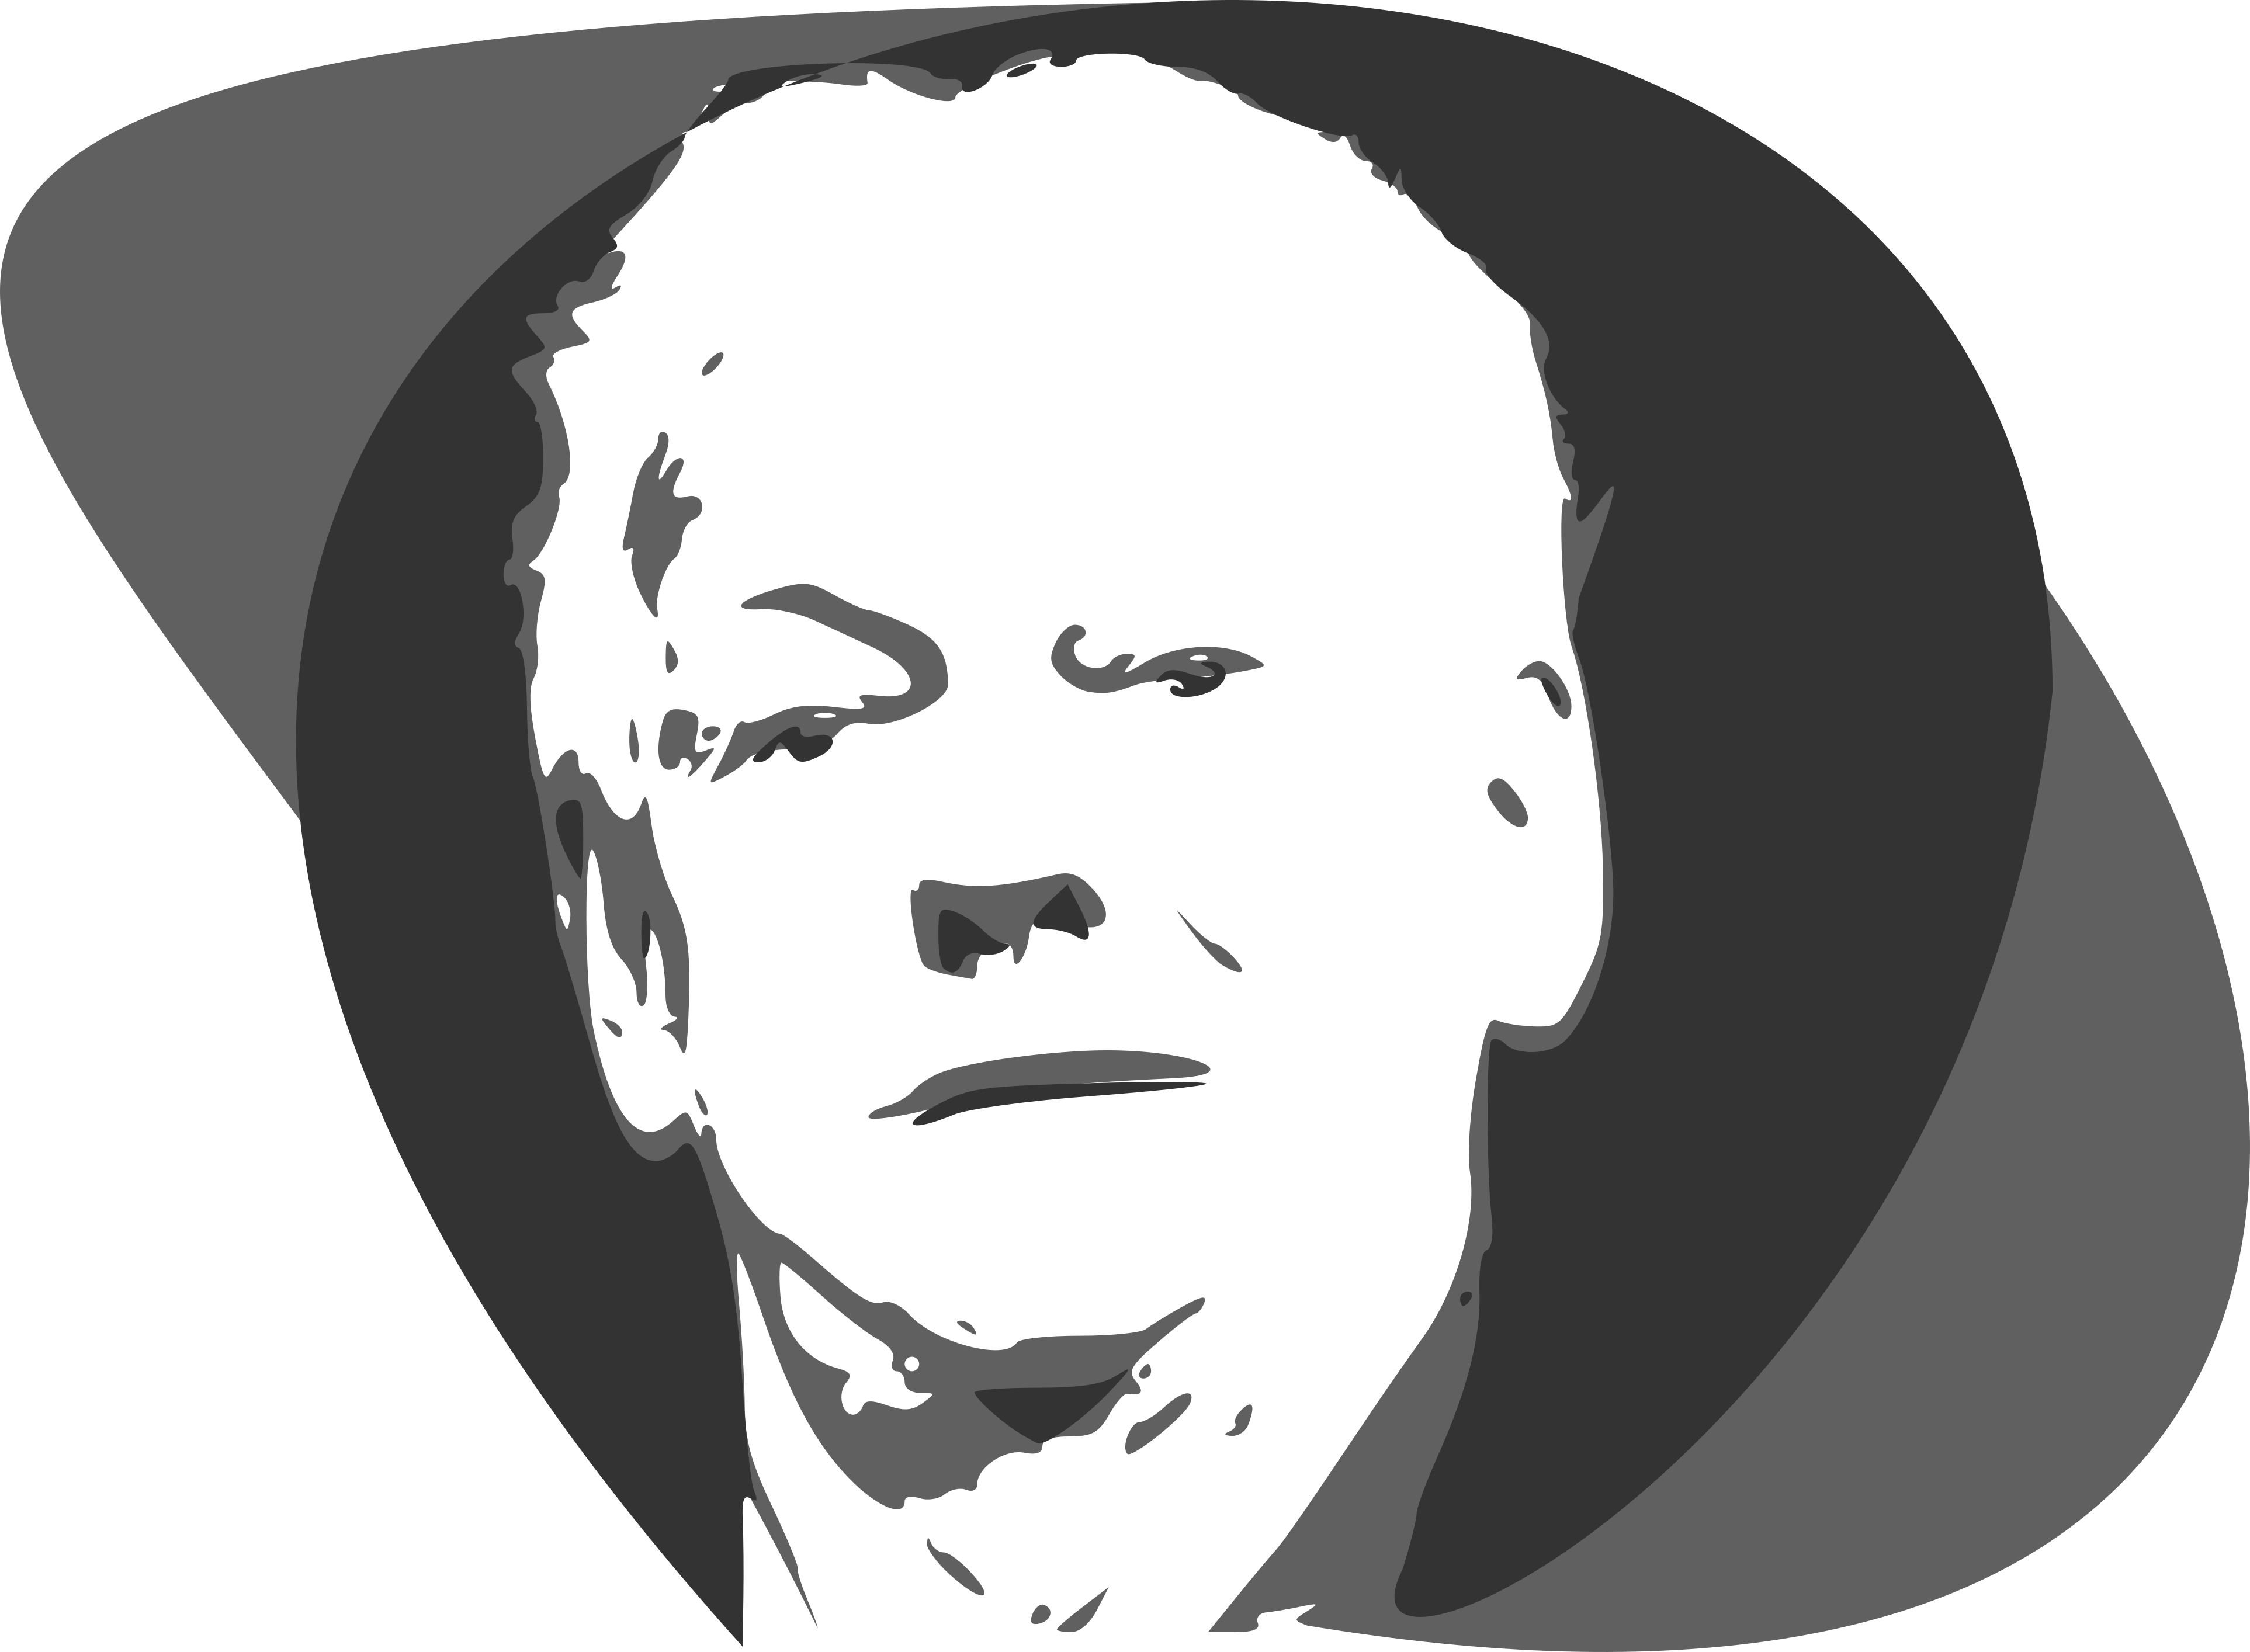
\includegraphics[width=\textwidth]{./bilder/wheterby.png}
\end{center}
\vspace*{\fill}
{\centering\fontsize{50}{48} \color{farbe}\sffamily{Wheterby Castle}\par}
\addcontentsline{toc}{chapter}{Wheterby Castle}
\newpage
%%%%%%%%%%%%%%%%%%%%%%%%%%%%%%%%%%%%%%%%%%%%%%%%%%%%%%%%%%%%%%%%%%%%%%%%%%%%%%%
\lettrine[lines=3, lhang=.2, loversize=.25, lraise=0.05, findent=0.1em,
nindent=0em]{D}{ie} Fahrt von London hat neun Stunden gedauert. Der Smog der Stadt geht fliessend in den Nebel vom Land über. Landschaft von nicht mehr als 20 Yard. Zugschwellen genen den Rythmus vor, verbieten jeden Gedanken. Tristesse und Trance im überhitzten Abteil. Von York aus nehme ich eine Kutsche in Richtung Küste. Schlaglöcher machen den Körper taub. Ich sollte für Lady Cantacuziono in London ein Stadthaus kaufen. Eine verwitwete rumänische Adlige, transsilvanischer Hochadel, sehr reich, mehr weiss ich nicht über sie. Ich habe einige Vorschläge, verschiedene Villen, ein kleines Schloss, Wohnungen in Kensington. Nachdem Geschäft sollte endlich das Gelfür die lange versprochenen Flitterwochen am Meer übrig sein. Die Hochzeit ist schon zwei Jahre her, die Erinnerung durch Alltag verblasst.

Der Kutscher bekreuzigt sich, als ich die Adresse nenne. \enquote{Seid ihr Christ? Dann nehmt dieses Kreuz.}, und reicht mir eine Kette, die fast ein Rosenkranz ist. \enquote{Das Haus ist verflucht, man sagt, dass alle die dort gewesen sind, entweder wahnsinnig wurden oder ganz verschwunden sind, überlegt es Euch gut, mein Herr.} 

Geschwätz mochte ich nie, Vorurteile kann ich mir nicht leisten. Es ist später Nachmittag als ich ankomme. Ein herrliches Schloss, historisierend gothisch, aber neu. \enquote{Sie hat einen Friedhof geschändet.} brummt der Fuhrwerker, Prim ausspuckend, brauner Schleim im Matsch. \enquote{Nun ja, nicht wirklich, aber Grabsteine für ertrunkene Seeleute haben hier gestanden, damit die Hinterbliebenen einen Ort zum Trauern haben. Ins Meer hat sie die geworfen.} Ihn ignorierend höre ich tatsächlich die See branden, tief unten an der Steilküste. Möwen schreien. Wenn ich das Meer sehe, habe ich Fernweh, schmecke Salz in der Luft. Kühler Wind, nicht stark, aber der Kraft, Armeen von Schiffen zu tragen. Mich an London erinnern, dessen Russ und Schmutz ich so liebe, ist hier unmöglich. Die Kutsche verschwindet im Nebel, mich alleine lassend.

Das schwere Tor ist geöffnet, der Garten wild, viele Rosen, in Hecken, als Büsche, rankend, blühend, verwelkt. Auf mein Klopfen reagiert niemand. \enquote{He}, rufe ich. Also stosse ich die Tür selber auf, trete ein, beklommen, ein Eindringling. Dabei sollte der Brief, der mich angekündigt hat, bereits hier sein. Ein grosser Saal, ein grosser Tisch, gedeckt für eine Person. Schweres Holz, Alter vortäuschend, als wäre es schon immer da gewesen. Gemälde bereits Verstorbener, Goldketten trangend, Zepter zur Schau stellend, Herschaflichkeit ausstrahelnd. Womit haben sie verdient, hier zu hämgen, was zeichnet sie aus?


Ein Zettel \enquote{Esst, ich stosse später zu Euch.}. Kaltes Huhn, fast roh, aber die Kartoffeln heiss und dampfend. Warum keine Bediensteten? Es ist unheimlich, ich schäme mich meiner, fühle mich falsch. Die Stille ist kaum zu ertragen. Aber die Reise war ermüdend, Hunger egalisiert anderes. Also esse ich. Der Wein ist fast schwarz, schmeckt tief und schwer, scheint sich im Hals aufzulösen, wird den Magen nie erreichen. Der beste, den ich je getrunken habe. In einem Zug leere ich den silbernen Becher, kann nicht absetzen.

\enquote{Ihr habt geschlafen.} Tatsächlich, meine Verwirrung ist vollkommen. Ich muss während des Essens eingeschlafen sein, warum erinnere ich mich an nichts? Das Huhn steht immer noch beinahe unagetastet vor mir. Es ist bereits dunkel, Kerzen erleuchten das Zimmer nur matt. Daher sehe ich sie nicht gleich, reibe mir verstört die Augen, aber noch steckt zu viel Schlaf in ihnen, um Schärfe zu erlauben.

\enquote{Willkommen auf Whetherby Castle. Ich bin Lady Cantacuziono.} Das Kreuz des Kutschers ist verschwunden, ich weiss es ohne in die Tasche zu greifen. Sie ist ganz in schwarz gekleidet, in tiefem Kontrast zu ihrer prozellanweissen Haut. Das Gesicht ist nicht zu erkennen. Seltsam langsame Bewegungen, fast verträumt. Sie nimmt eine Nuss aus einer Schale, umschliesst sie mit zarten Fingern und knackt sie, als wäre dies die natürlichste Art. Wie die Nuss in ihren Mund gelangt, verstehe ich nicht.

\enquote{Ich habe sie erwartet}. Ich stehe endlich auf, erschrocken von meiner Unhöflichkeit, verbeuge mich, gebe ihr die Hand. Wie kalt sie ist. Ich erkläre mich, stammele wie peinlich mir es sei, eingeschlafen zu sein, mit einer angedeuteten Geste deutet sie mir aufzuhören. Ich spüre wie mir Schweiss den Rücken herabläuft, bin verlegen, verunsichert.

\enquote{Wenn sie wünschen kann ich ihnen gerne die Unterlagen geben, ich habe verschiedene Optionen für sie ausgewählt\dots} 

\enquote{Sie werden mir ein Haus kaufen, ich bin an Optionen nicht interessiert.}, weist sie mich zurück. Sagt sie das wirklich oder meine ich es nur zu hören? Es muss an diesem Schlaf liegen, der nicht verschwinden will, aber warum kann ich die Frau nur undeutlich sehen? Mein Blick verschwimmt, aber nur bei Ihr. Den fetten Mann auf dem riesigen Bild sehe ich, Goldene Knöpfe auf der Brust,aber sie? Wie der Rauch einer erlöschenden Kerze.

\enquote{Erlauben sie mir eine Frage}, setze ich an, will wissen, warum es keine Diener gibt, weswegen ich mich so eigenartig fühle, aber sie verneint bevor ich die Frage stellen kann mit einer Geste, die ich nicht kenne aber verstehe. Pachuli. Ein schwerer Geruch umströmt sie, wird mir jetzt bewusst, erreicht mich, dringt auch in mich ein. Ich muss endlich aufhören zu träumen, muss mich fokussieren, kann es aber nicht. Werde immer tiefer hinabgezogen. Sand zerrieselt zwischen meinen Fingern. Ich entschuldige mich stotternd, versuche die Fassung zu wahren. War sie eben auch schon so riesig? Sie scheint den Raum vollständig auszufüllen, ist dabei aber weiter zerbrechlich zart, elegant. Ihr Anblick verweht, wenn ich ihn fassen will, sie ist überall und doch nicht da. Ich spüre ihre glatte und zarte Haut.

Ich stütze mich auf den Tisch, der Schweiss tropft mir aus den Haaren, wie finde ich mich wieder? Sie führt mich in ein Zimmer, ich schlottere, kann mir nicht helfen. Dass sie mir zwei riesige Hunde zu meinem Schutz da lässt, nehme ich nicht wahr. Gross und drohend sitzen sie vor meinem Bett, in das ich sinke ohne die Kleider zu wechseln. Sie werden die ganze Nacht knurren und am Morgen verschwunden sein. Ich schlafe nicht, träume nur. Der einzige Mitgefangene in meinem kleinen Kerker ist meine Angst. Schwarz und kalt. Einsamkeit, Verlassensein, Leere. Als endlich die Sonne aufgeht stehe ich auf, bin wieder alleine in dem Schloss. Die Nacht ist vorbei, ich weiss wieder wer ich bin, was ich bin. 

Ein unterschriebener Kaufvertrag liegt auf dem Tisch, von draussen ruft ein Kutscher. 
